
\chapter[Approach]{Approach}
\graphicspath{ {images/approach} }

In this chapter we present the approach that we developed to visualize software system using a visual and auditive depiction of the evolution of a system. 
To do that, we have chosen to leverage on the phenomenom of the Synesthesia, the production of a sense impression relating to one sense by stimulation of another sense.
.....





Our approach consists of two parts:
In the first part we modelled the evolution of the software artifacts, and we enginereed a tool that implement it.
In the second part, we used the concept of synesthesia (the production of a sense impression relating to one sense by stimulation of another sense) 
to enhance the effectiveness of the visualization. 

Comprehending the evolution of a software system is difficult, mostly for the sheer amount of data and its complexity. 
The term "software evolution" was conied for the first time by Lehman in 1985 in a set of laws. \cite{Lehman1985}
He stated that the complexity of a system is destinated to increase overtime, as the system always needs to be adapted to its evolutionary environments. 
To be managed, software systems needs to be compprehended by developers, and this activity can be simplified with software visualization. 

..


To visualize the evoluton of a system, there are many aspects that we can consider. \\
\bigbreak

In our approach we focus on systems that resides on git repositories. 
We made this choiche because git is the most common repository management system and it also track all the changes made to every file of the system.
So, every git repository holds the whole history of a software system.\\
\\

In our approach, we model the evolution of repository files, therefore we model its history. 
To do that, we considered all the information that can be extracted from a git repository: files and commits.

The git protocol is responsible for tracking the changes made to the system.
To do that, every time we made a commit, it stores only a list of files that have been modified. 
Every commit is represented by a tree of hashes, each one representing a file. 

Git has the possibility to inspect every commit of a repository by using the command \texttt{git checkout}. 
In this way, we can navigate through the history of a repository, to track all the files, their changes and their metrics.\\

A commit operation contains also other meta-information such as the author, the date and the message. 



\section{Evolution Model}

\begin{figure}[H]
    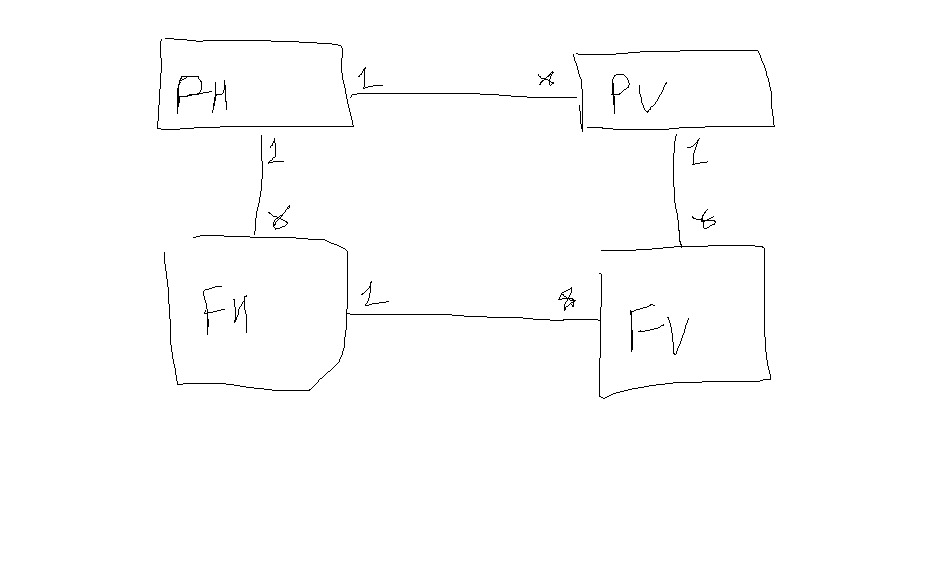
\includegraphics[width=0.6\textwidth]{EvolutionaryModel.jpg}
    \caption{Evolutionary Model}
    \label{fig:EvolutionaryModel1}
\end{figure}

To model the evoltion of software systems, we delveloped a new model, 
showed in figure \ref{fig:EvolutionaryModel1}, based on Hismo, a solution presented by Tudor Girba \cite{Girba2005}.\\
\\
The needed to develop a new evolutionary comes from the fact that Hismo was developed to work with another versioning system: Subversion (SVN). 
There are several difference between SVN and git. The most important, in terms of design, is on how they keep track of changes. 
In fact, SVN works with the concept of snapshot. Every time a developer changes some files, committing theese changes, it will increase the revision of the whole system. 
In constrast, git, only the modified files would get the version field updated. 
Therefore, we need to adapt our model to work well with git because the Hismo model is based on three main entities:
\begin{itemize}
    \item Snapshot. A representation of the entity whose evolution is studied.
    \item Version. An entity that adds the notion of time to a Snapshot by relating it to the History. 
    \item History. An entity that holds of a set of Versions.
\end{itemize}
\bigbreak

Since in git we don't have the concept of Snapshot, we needed to replace it with file versions. 
A file version is essentially the version of a file in a particular point in time. 
It is associated with a project version, that set the time and with a file history, that set the file that has been updated.
To summarize, the main entities of our model are: 
\begin{itemize}
    \item \textbf{ProjectHistory}: it represents the repository of a system. It is an holder of two sets: FileHistories and ProjectVersions. 
    \item \textbf{FileHistory}: it represents a file in the whole history of the repository.
     If a file has been renamed or moved, the entity representing that file will remain the same.
     So, it is resilient to renaming and moving activities. 
     It holds a set of FileVersions, that represents the version of the entity in a particular point in time. 
    \item \textbf{ProjectVersion}: it represents a commit or a version of the system. 
    For each changed file inside a commit, the respective ProjectVersion contains a FileVersion representing that change.
    A ProjectVersion also holds contextual information about the commit such as the timestamp, the hash of the commit and the message.
    \item \textbf{FileVersion}: it represents the version of an entity in a particular point in time.
    It is responsible to hold all evolutionary information of an entity, since it represent an evolutionary step of that entity. 
\end{itemize}
\bigbreak

\subsection*{Historical information retrival}
To build the history of a repository, we need to extract the historical information from git.\\
To understand better how we approached to it, we have to explain how git internally represents the repository history. 
Git works with the concept of branches, each branch can be seen as a different timeline of the repository.
Usually, developers exploit branches to develop features on it and then merge the developed code with the existing codebase.
To do that, they need to create a commit called "merge commit". 
Each time we create a new git commit, we are deploying a new version of the system, that records all the changes made to the commits's tracked files. 
Internally, in git, all the commits are stored as nodes of a tree called commit-tree. 
The root node represents first commit of the repository, since it has not any parents. 
All the other nodes instead, represent the commits made during the whole lifecycle of the repository. 
Each commit usually have only one parent, that represents the previous commit made before that one.
There is one case where a commit might have more than one parent: merges commits.
\bigbreak
As a convention, each repository should has a branch that should contain the stable, production-ready code. Usually this branch is named "main" or "master". 
In our approach, we aim to analyze the timeline of this branch. To do that, we start from the first commit present in the repository history, and then we traverse the whole commit tree. 
However, during this proccess, we don't consider merge commits, since they incorporate commits already made, and thus they would be considered twice. 
Once we have extracted all the valid commits, that resides on the main branches, we need to take from them all the representative information that we need for a project version. \\
\bigbreak
Git, is able to recognize the following actions made on a file:
\begin{itemize}
    \item \textbf{ADD}. A file is to the repository.
    \item \textbf{DELETE}. A file is has been removed from the repository.
    \item \textbf{MODIFY}. A file is has been modified.
    \item \textbf{RENAME}. A file name has been changed. Wheater the filepath has been changed, the parent directory path must remain the same. 
    \item \textbf{MOVE}. A file was moved from one location to another, so the file path has been changed. This action is detected wheter the filename remained the same. 
\end{itemize}

From a commit we could also extract additional information such as the name of the file being modified, the parent directory, the number of lines added and removed, the path of the file before and affter the changes and many more.
We used the commit's information to track all the paths of an entity. In this way, we can update the entity path when it was renamed or moved to track it during all its lifecycle. \\
\linebreak
When we reconstruct the history of a repository, each FileHistory starts with a FileVersion representing an ADD action. Then, in the middle of the FileVersion set we can find only three kind of actions: MODIFY, RENAME and MOVE. 
In some cases an entity might be deleted, so the last FileVersion holded by a FileHistory will represent a DELETE action. 

\begin{figure}
    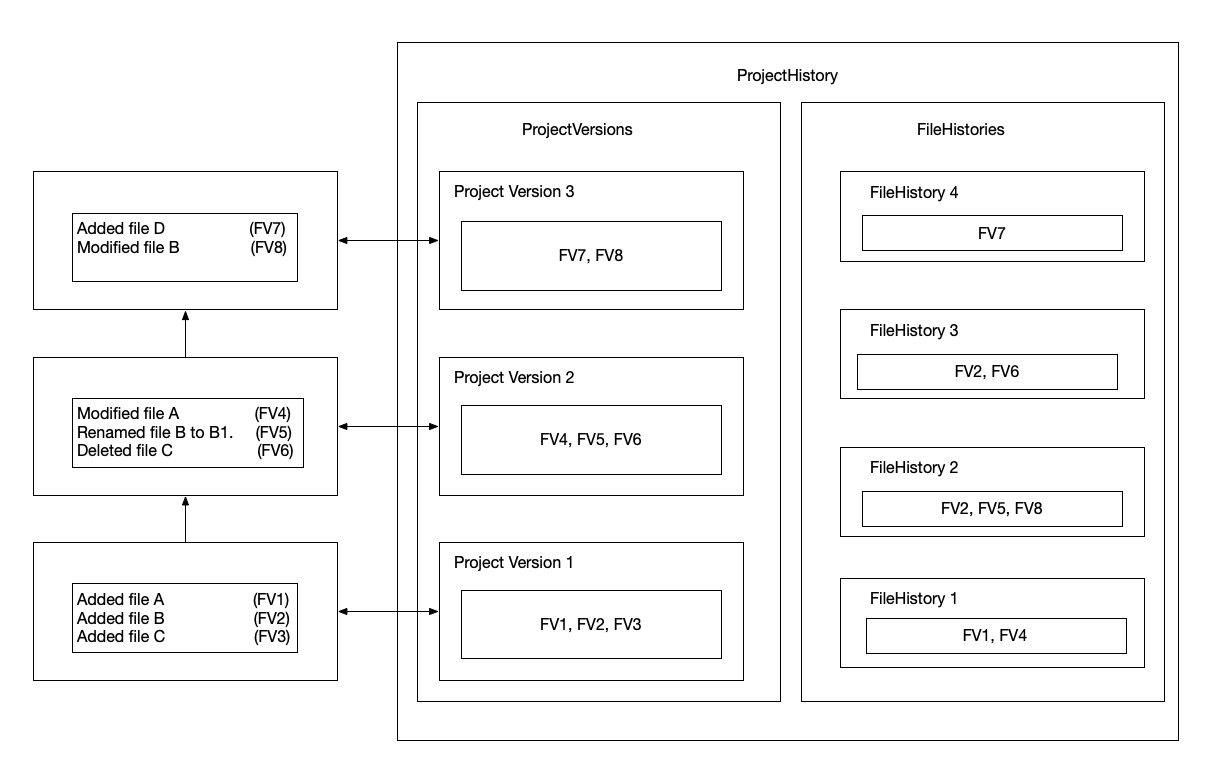
\includegraphics[width=0.6\textwidth]{ApproachExample.png}
    \caption{Rebuilding history example}
    \label{fig:ApproachExample}
\end{figure}

Figure \ref{fig:ApproachExample} shows an exaple of how history is rebuilt. 
First we create a ProjectHistory that holds a set of ProjectVersions and a set of FileHistories. 
After that, we start to traverse the repository's commit tree.
As we can notice, for each commit we create a new ProjectVersion. It represents a new version of the system in our model. 
Therefore, we inspect the commit's changelist and we create a new ProjectVersion for each entry of the list.
With this operation, we can discover if a file has been added to the system, because on that case the change should represent an ADD operation and thus we can create a new FileHistory. 
At version 1, three new files were added to the repository (A, B, B) and, as we can see, three new FileHistories were created. 
Each chage was mapped to a FileVersion (FV), then we added them to the Respective FileHistory and ProjectVersion. 

 



\section{Visualization}

\subsection*{2D representation}
This model, could be also representd by a 2D matrix. 


From our point of view, a file can be seen as an holder of file versions.
A file version represents a file in a particular point of time. The difference between a file version a


As a consequence, our new model, depicts every File in the system, as an holder of a set of FileVersions. 
The File entity, named to be consistent with its scope as FileHistory, is stored on another entity called ProjectHistory, that follows the same logic. 
In fact a ProjectHistory is no less than a holder of two sets: one for the FileHistories and one for the Versions. 




\begin{itemize}
    \item Each column of the matrix represent a commit, a version of the software.
    \item Each row of the matrix represent a file, named FileHistory.
    \item Each cell of the matrix represent the different versions of a file. Empty cells represent a file that has not been modified.
    \item A file can have multiple names (tollerant to renaming and moving operations).
    \item Files are sorted by addition time, on the top we will have all the files that were added in the first commit of the repository. 
\end{itemize}

For now on, we will use the following notation:


Therefore, a FileHisory represents the history of an entity of our system. 
The name of the file is not a concern for us, until a file is not deleted it will always represent the same entity. 


And we will use them in our model to identify the action associated to a FileVersion. 
\begin{figure}
    \center
    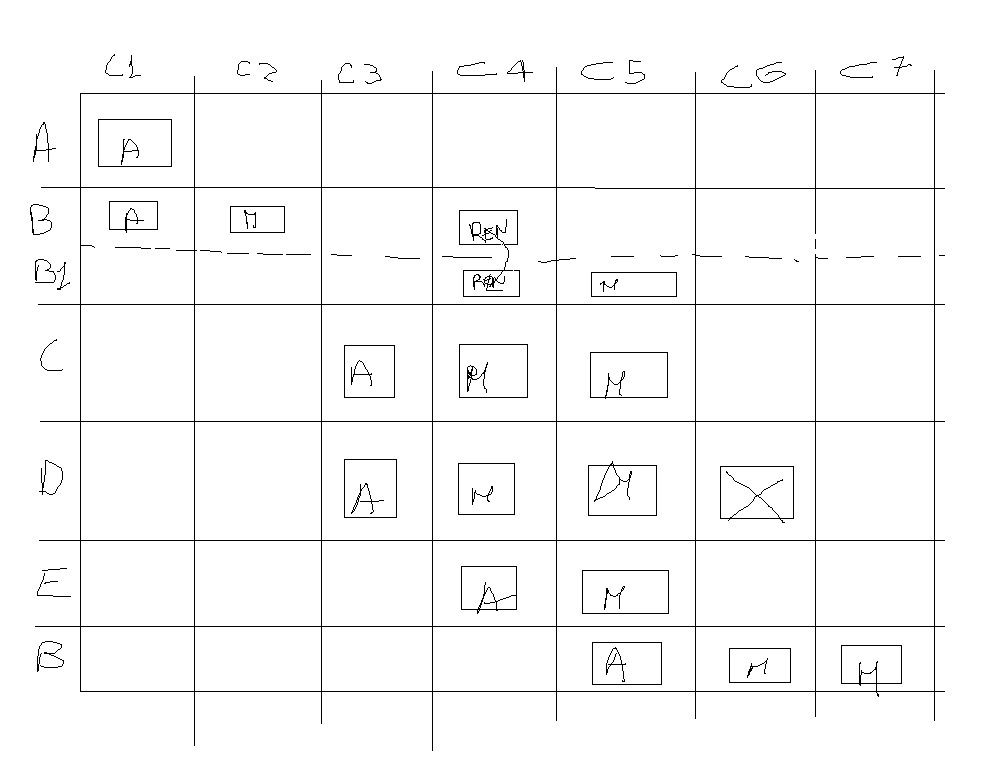
\includegraphics[width=0.6\textwidth]{ApproachMatrix.jpg}
    \caption{Evolution matrix of a repository}
    \label{fig:evolutionMatrixApproach}
\end{figure}
Figure \ref{fig:evolutionMatrixApproach} present a schematic evolution matrix of a repository with seven versions.
As we can see, in the first ProjectVersion, there were added two files, A and B. In the second revision B was modified, and in the third revision C and D were added.
The fourth revision recorded a rename of B to B1.
It's important to notice that B and B1 represent the same entity, therefore they are represented by the same FileHistory.\\



Based on our aim, we can read this matrix as follows:
 \begin{itemize}
     \item \textbf{by rows}, if we are intrested on the history of a particular entity of our system. 
     For examle, the FileHistory represented by the first third row in figure \ref{fig:evolutionMatrixApproach}, represents the history of the file D. 
     The file D was added in the third ProjectVersion (so the third commit), modified in the fourth and fifth ProjectVersion, and then deleted in the sixth ProjectVersion.
     The figure \ref{fig:evolutionMatrixApproach} is also a good exaple to understand why we cannot rely on the name of the file to identify the entity. 
     We can notice that the file B represented by the second FileHistory, was added on the first version and then renamed on the fourth from B to B1. 
     Then, in the fifth version, a new file called B was added. Nonetheless the name of the files are the same, they must represent two different entity. 
     We would have had the same result, even if the file B was been added in the version four. 
     \item \textbf{by columns}, if we are intrested on which entities were updated on each ProjectVersion. 
    For example, on the first ProjectVersion we have added the first and the second entity. 
    On the fourth ProjectVersion we have renamed the second entity, we have modified both the third and the fourth, and finally we have added the fifth entity.
 \end{itemize}

\begin{figure}
    \center
    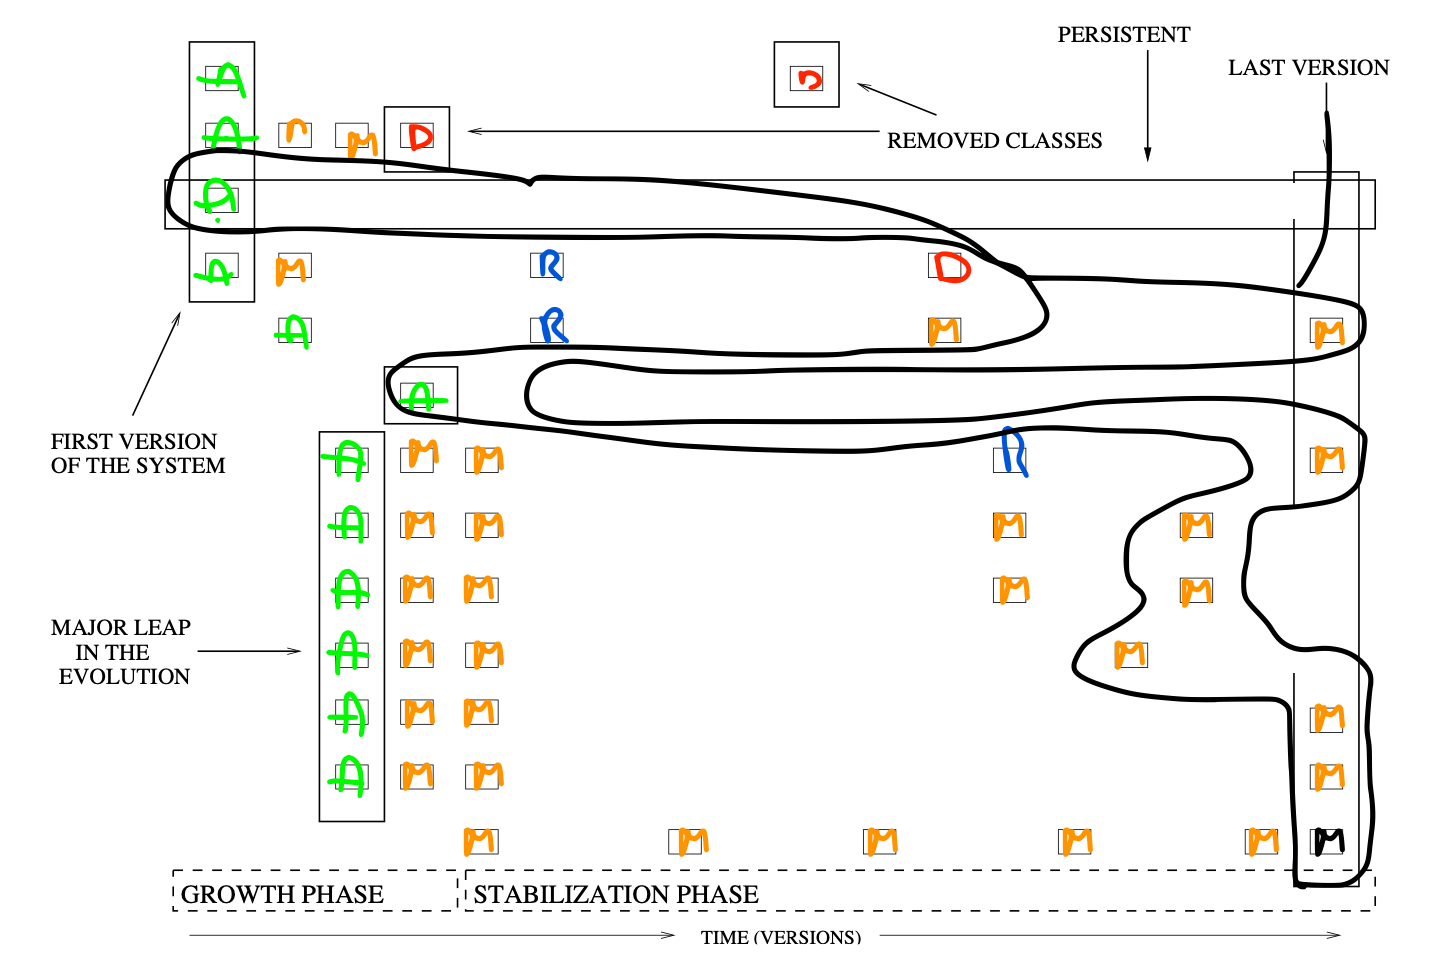
\includegraphics[width=\textwidth]{ApproachMatrix2.png}
    \caption{Evolution matrix of a repository}
    \label{fig:evolutionMatrixApproach2}
\end{figure}

Figure  \ref{fig:evolutionMatrixApproach2} shows an exaple of how to recover evolution information from the matrix. 
As we have seen, each version doesn not represent a snapshot of the system.
Instead it represents only the differentce in term of changes made to the previous version. 
Given that, to recover a snapshot of a specific version, we need to consider the last changes made before that specific version.
Under those circumstances, for each FileHistory, we need to go back in time until we find the leftmost change. Of course, if the leftmost change was a delete, we have to ignore the releated FileHistory.
In contrast, if we have to display the evolution of a snapshot, we need to consider only the changes made after that snapshot. 
So, each time we need to display a ProjectVersion, we have to take all its FileVersions and merge them with the current state of the snapshot. 

\subsection*{3D representation}

Software systems are hard to understand due to the complexity and the sheer size of the data to be analyzed.
Our approach aims to make the analysis of a system easier for engineers, through the exploitation of the human senses.
This is the reason why we have chosen to leverage on the phenomenom of the Synesthesia.
The phenomenon of the synesthesia occurs  when a stimulation of a sense or a cognitive pathway leads to the involountarly stimuation of another sense or a cognitive pathway.
We experience synesthesia when two or more things are perceived as the same. 
For exaple, synesthetic people might associate the red color with the letter D or the green color with the letter A. 
There are many forms of synesthesia, each one representing a different type of perception, such as visual forms, auditory, tactile, etc.\\
\\
In our approach we use the following visual aspects to trigger involountarly associations:
\begin{itemize}
    \item \textbf{Color}: we use the color of the entity to describe the last action made on that entity.
    \item \textbf{Shape}: we use the shape of the entity to describe the type of the entity. 
    For exaple, a java file could be represented by a cube whereas a binary file could be represented by a sphere.
    \item \textbf{Height}: we use the height of the entity to describe the value of a representative metric, used to compare entities.
\end{itemize}
Entities are displayed with an outward spiral layout to emphatize their order on the evolution matrix. \\
\\
There are several ways to traverse the history of a repository. 
The visualization needs to start from the first moment and then go forward until the end. The question is, how we should go forward in time?
We came up with two strategies: 
\begin{itemize}
    \item We can display \texttt{n} version at time, so we are traversing the history as it was written. 
    A limitation of this approach is that we lose the concept of time. 
    We cannot have any idea about how much time was passed between two commit, thus we cannot distinguish active development phases from unactive development phases. 

    \item We can group version by their timestamp. So, all the commit made in the sime time period, will be displayed at the same time. 
    This strategy works very well if we need to comphrend how the system evolved and at which speed in time. 
\end{itemize}

We conchretized our strategies within the concept of \textbf{moment}. A moment is a group of version that will be displayed at the same time. 


\begin{figure}[H]
    \begin{center}
        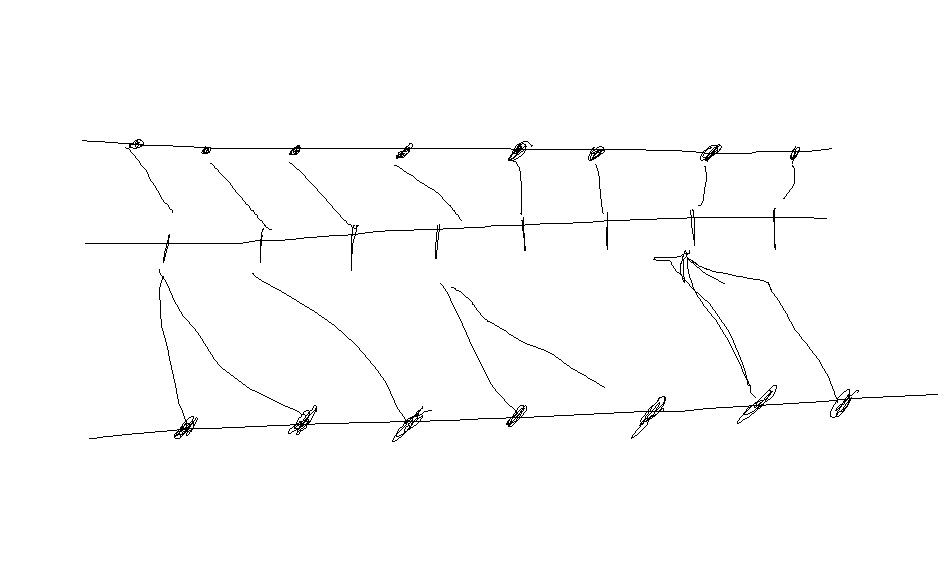
\includegraphics[width=0.9\linewidth]{Moments.jpg} 
        \caption{Example of two different strategies to identity moments. 
        On the first strategy, we mapped one commit with one moment, so the total number of moments will be equals to the total number of commit.  
        Alternatively, on the second strategy, we created a moment every day.
        As a result, we have some moments with many commits, and some without anyone.
        With this strategy, the number of moments will be the same as the number of days that have passed between the first and the last commit. 
        }
        \label{fig:moment}
    \end{center}
\end{figure}

Figure \ref{fig:moment} highlights the difference between the two strategies mentioned above. 


\subsection*{Color}


\begin{wrapfigure}{r}{0.3\textwidth}
    \begin{center}
        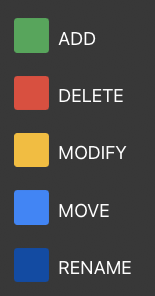
\includegraphics[width=0.7\linewidth]{ColorAssociation.png} 
        \caption{Color association}
        \label{fig:ColorAssociation}
    \end{center}
\end{wrapfigure}

The color of the entity should recall the last action made on that entity. To achieve this purpose, we used the color association described in figure \ref{fig:ColorAssociation}.
Nonetheless, each person has its own perception of colors, thus, we can not assume that this color will work in the same way for all the pepoles.
To remedy this issue, users can customize the color palette as they wish. \\
\\
We decided to put another information on the color of the entity: the \textbf{aging}. 
We define the aging of an entity as the number of moments since the last modification of that entity happened.
To do that, we mapped the age of an entity with the darkness of its color. 
As a result, older entities will be displayed with a darker color. 
In this way, users can immediately recognize the last action and the amount of time passed since the entity was modified.


\subsection*{Shape}
We have chosen to play with the shape of the entity to distinguish them based on their type. 
Our visualization layour works with an ourward spiral, that always adds a new entity at the tail. 
If a commit involves lots of entities, it would be useful to know immediately, which kind of entities are been modified. 
For this reason, we mapped the shape of the entity to the file type of the entity itself.
Usually, in a repository, there are many file types, so we cannot aim to have a exhaustive set of shapes, to represent each file type individually. 
Therefore, we have defined a taxonomy

\subsection*{Height}
The height of an entity should represent the value of a metric.


\section{Auditive model}